%%%%%%%%%%%%%%%%%%%%%%%%%%%%%%%%%%%%%%%%%%%%%%%%%%%%%%%%
%   |------------------------------------------|       %
%   | Web App embebida en dispositivos móviles |       %
%   |  para la gestión de registros sobre la   |       %
%   |   contaminación de afluentes y ríos.     |       %
%   |                                          |       %
%   |          Proyecto de graduación          |       %
%   |__________________________________________|       %
%                                                      %
%   Autores                                            %
%   -------                                            %
%                                                      %
% * Bruno, Ricardo Hugo (CX 1409686)                   %
%     rburnount@gmail.com                              %
% * Gomez Veliz, Kevin Shionen (CX 1411828)            %
%     ing.gomezvelizkevin@gmail.com                    %
%                                                      %
%   Tutor                                              %
%   -------                                            %
%                                                      %
% * Ing. Cohen, Daniel Eduardo                         %
%        dcohen.tuc@gmail.com                          %
%                                                      %
%   Cotutor                                            %
%   -------                                            %
%                                                      %
% * Ing. Nieto, Luis Eduardo                           %
%        lnieto@herrera.unt.edu.ar                     %
%                                                      %
%                                                      %
%%%%%%%%%%%%%%%%%%%%%%%%%%%%%%%%%%%%%%%%%%%%%%%%%%%%%%%%

\chapter{Disciplina de Análisis}
\label{chap:analisis}

\section{Vista de Casos de Uso}

La vista de casos de uso captura el comportamiento de un sistema, subsistema, clase o componente, como lo ve un usuario externo. Particiona la funcionalidad del sistema en transacciones significativas para los actores (usuarios idealizados) de un sistema. Las piezas de funcionalidad interactiva son llamadas ``casos de uso''. Un caso de uso describe una interacción entre actores como una secuencia de mensajes entre el sistema y uno o más actores. El término \emph{actor} incluye a personas, como también otros sistemas de computadora o procesos.

\section{Diagrama de Contexto}

\begin{figure}[H]
  \centering
   
    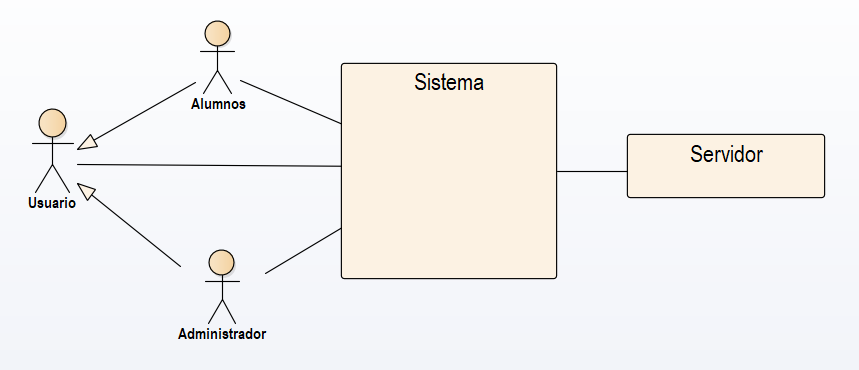
\includegraphics[width=1\textwidth]{imagenes/analisis/diagrama-contexto.png}
        %%Me parece que queda mejor sin el hfill
        %\hfill
    %\caption{epígrafe}
	\label{fig:casos-de-uso}
\end{figure}

\section{Diagramas de Casos de Uso}

Primeramente se muestra un diagrama de caso de uso general donde se agruparon los casos de uso por las acciones en común, luego se va a explorar cada caso de uso de manera mas descriptiva.

Por ejemplo, en ``Gestión de Registros'' van a estar todos los casos de uso referidos a los mismos (alta, baja, listar, buscar, etc)

\subsection{Diagrama de Casos de Uso general}

\begin{figure}[H]
  \centering
    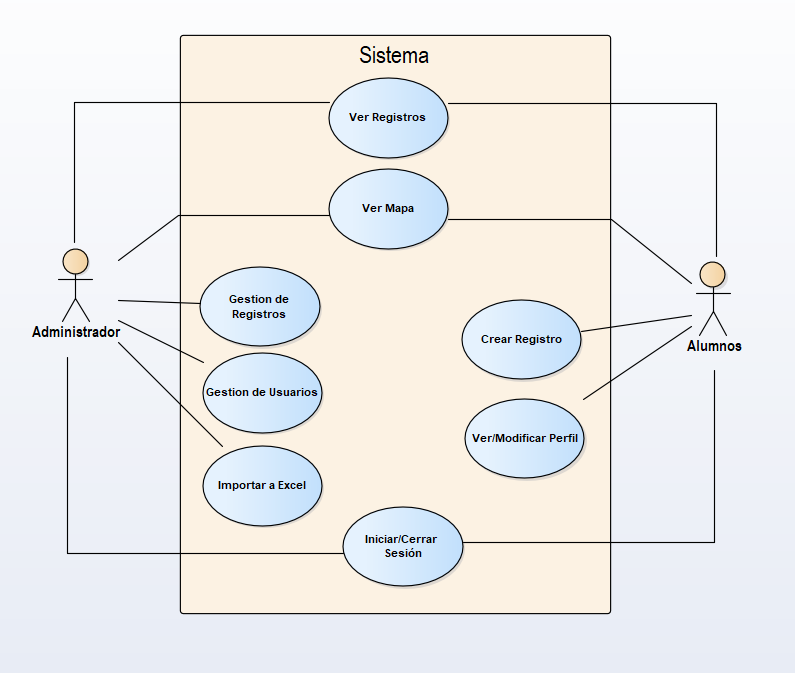
\includegraphics[width=0.7\textwidth]{imagenes/analisis/casos-uso-general.png}
        %%Me parece que queda mejor sin el hfill
        %\hfill
	%\caption{epígrafe}
	\label{fig:casos-de-uso}
\end{figure}

% \subsection{Diagrama de Casos de Uso de gestión de usuarios}

% \begin{figure}[H]
%   \centering
%     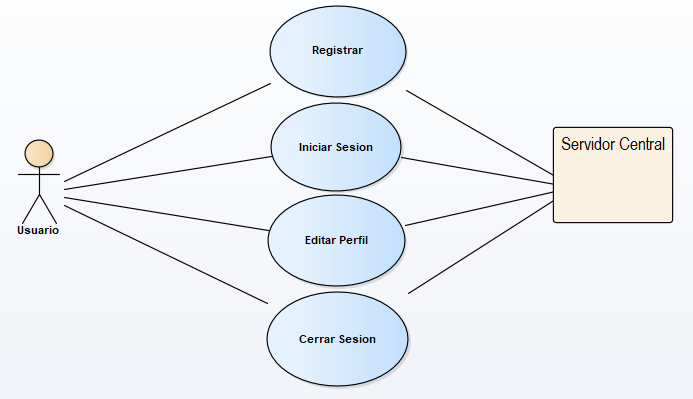
\includegraphics[width=0.7\textwidth]{imagenes/analisis/casos-uso-usuario.png}
%         %%Me parece que queda mejor sin el hfill
%         %\hfill
%     %\caption{epígrafe}
% 	\label{fig:casos-de-uso-usuario}
% \end{figure}

% \subsection{Diagrama de Casos de Uso de gestión de tienda}

% \begin{figure}[H]
%   \centering
%     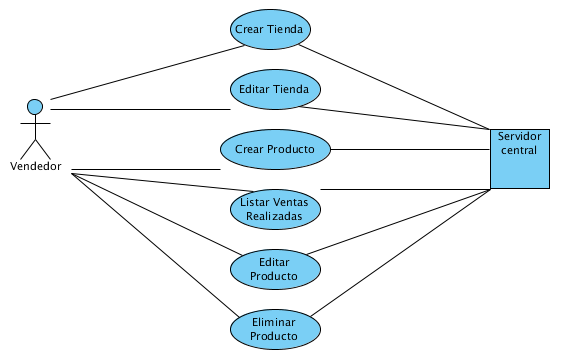
\includegraphics[width=0.7\textwidth]{imagenes/analisis/casos-uso-tienda.png}
%         %%Me parece que queda mejor sin el hfill
%         %\hfill
%     %\caption{epígrafe}
%     \label{fig:casos-de-uso-tienda}
% \end{figure}


% \section{Diagramas de Actividad}

% \subsection{Autenticar}
% \begin{figure}[H]
%   \centering
%     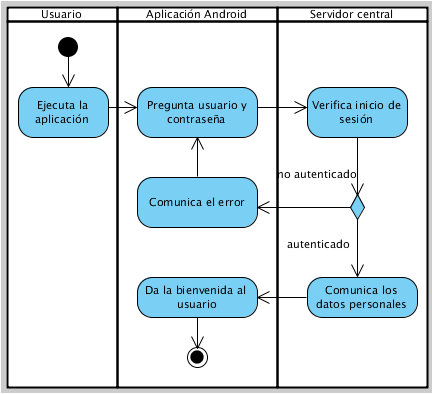
\includegraphics{imagenes/analisis/diagrama-actividad-autenticar.png}
%         %%Me parece que queda mejor sin el hfill
%         %\hfill
%     \label{fig:diagrama-actividad-autenticar}
% \end{figure}

% \subsection{Registrar}

% \begin{figure}[H]
%   \centering
%     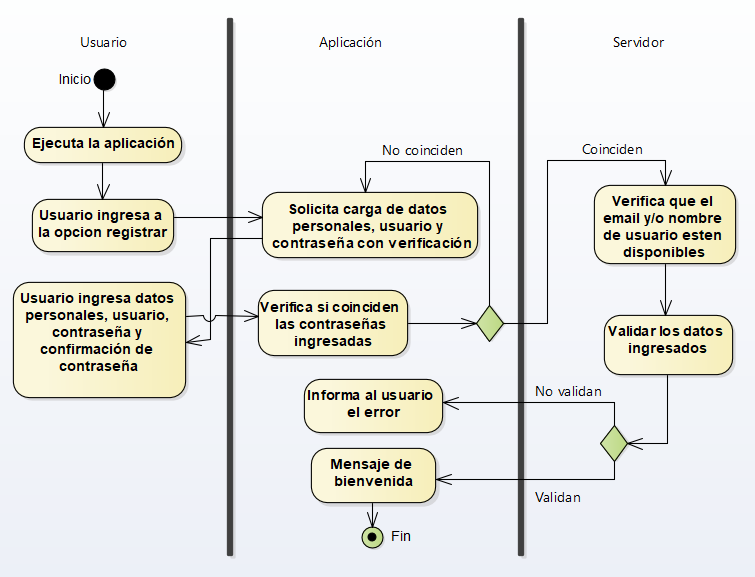
\includegraphics[width=1\textwidth]{imagenes/analisis/diagrama-actividad-registrar.png}
%         %%Me parece que queda mejor sin el hfill
%         %\hfill
% 	\label{fig:diagrama-actividad-registrar}
% \end{figure}

% \subsection{Crear Tienda}

% \begin{figure}[H]
%   \centering
%     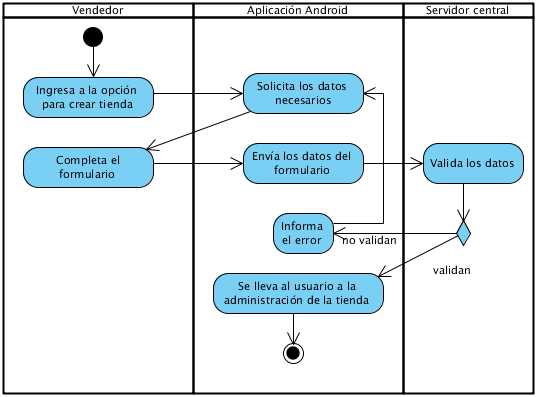
\includegraphics{imagenes/analisis/diagrama-actividad-crear-tienda.png}
%         %%Me parece que queda mejor sin el hfill
%         %\hfill
%     \label{fig:diagrama-actividad-crear-tienda}
% \end{figure}

% \subsection{Comprar Producto}

% \begin{figure}[H]
%   \centering
%     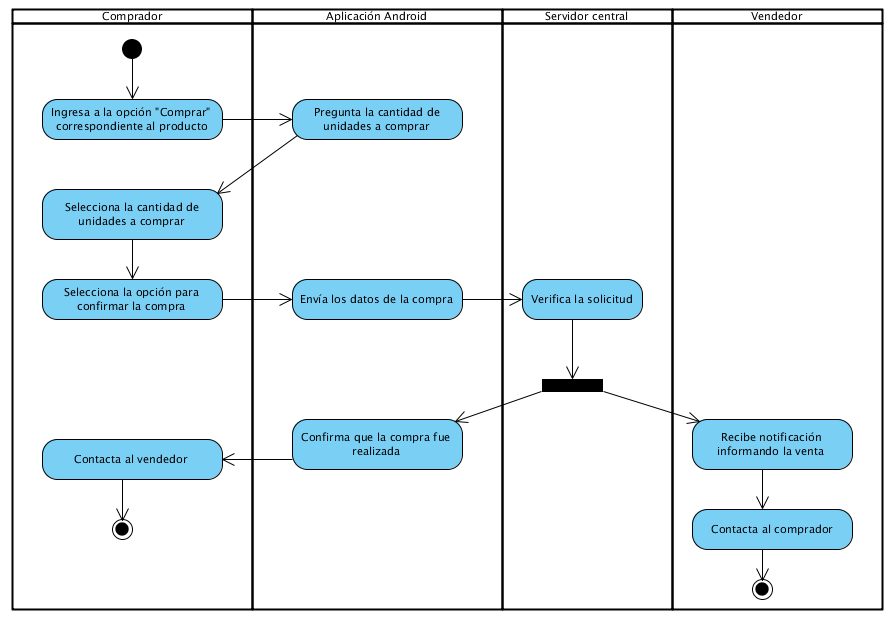
\includegraphics[width=1\textwidth]{imagenes/analisis/actividad-comprar-producto.png}
%         %%Me parece que queda mejor sin el hfill
%         %\hfill
%     \label{fig:diagrama-actividad-comprar-producto}
% \end{figure}

\newpage
\subsection{Casos de Uso Principales}

\begin{enumerate}
    \itemsep-1em
    \item Un alumno no registrado desea registrarse en el sistema.
    \item Un alumno registrado desea iniciar sesión.
    \item Un alumno registrado desea crear un registro.
    \item Un alumno registrado desea ver un registro en particular.
    \item Un alumno registrado desea ver el mapa general.
    \item Un alumno registrado desea ver su perfil.
    \item Un alumno registrado desea modificar su perfil.
    \item Un alumno registrado desea cerrar sesión.
    \item Un alumno registrado desea eliminar su cuenta.
    \item Un administrador desea iniciar sesión.
    \item Un administrador desea borrar o dar de baja un alumno.
    \item Un administrador desea listar los alumnos.
    \item Un administrador desea listar los registros.
    \item Un administrador desea aprobar o rechazar registros.
    \item Un administrador desea ver un registro en particular.
    \item Un administrador desea buscar registros por fecha de creación.
    \item Un administrador desea buscar registros por institución.
    \item Un administrador desea buscar registros por indice.
    \item Un administrador desea ver el mapa general.
    \item Un administrador desea exportar a Excel la información.
    \item Un administrador desea cerrar sesión.


\end{enumerate}